% TODO: Отступы до и после формул, нужно это закинуть в `spbseu.cls`
\setlength{\abovedisplayskip}{1.5mm}
\setlength{\belowdisplayskip}{1.5mm}


\section{Задачи, решаемые методом динамического программирования}

\indent Особенность производственных задач, решаемых методом динамического программирования, заключается в том, что процесс, протекающий в системе, зависит либо от времени (от этапов), либо имеет многоступенчатую структуру. Метод решения задач динамического программирования состоит в том, что оптимальное управление строится поэтапно шаг за шагом. На каждом этапе оптимизируется только один шаг, но при этом учитывается изменение всего процесса, так как управление, оптимизирующее целевую функцию только для данного шага, может привести к неоптимальному эффекту всего процесса. Управление на каждом шаге должно быть оптимальным с точки зрения процесса в целом.

В основе вычислительных алгоритмов динамического программирования лежит принцип оптимальности Р. Беллмана. (Формула \ref{eq:bellman}) Данный принцип включается в себя три основных этапа:
\begin{enumerate}
    \item предварительный этап;
    \item этап условной оптимизации;
    \item этап безусловной оптимизации.
\end{enumerate}

Предварительный этап проводится с целью уменьшения вычислительной работы на последующем этапе решения и, по существу, заключается в нахождении всех допустимых значений управлений $u_i$ и фазовых переменных $x_i$, то есть фактически область определения функций $B_i(x_i)$ или, в более сложных случаях, множеств, содержащих эти области определения. Иными словами, на данном этапе отбрасываются все заведомо неподходящие, нереализуемые значения фазовых и управляющих переменных. Проводится предварительный этап в естественном порядке от первого шага к последнему: $i = 1, 2, \hdots, n$, а опираются соответствующие расчёты на уравнение процесса $x_i = f_i(x_{i−1},u_i)$. Данный этап особенно удобен при табличном способе задания функций, фигурирующих в условии задачи.

Условная оптимизация осуществляется поэтапно при движении из конечного состояния $x_n$ системы $S$ в первоначальное состояние $x_0$ путём построения на каждом этапе условно-оптимального управления и нахождения условно-оптимального значения функции цели для каждого шага.

Безусловная оптимизация осуществляется в обратном направлении: от первого шага к последнему, в результате чего находятся уже оптимальные управления на каждом шаге с точки зрения всего процесса. На втором этапе отрабатываются рекомендации, полученные на этапе условной оптимизации.

Много интересных многошаговых процессов принятия решений возникает при управлении производственными процессами. Рассмотрим некоторые из них.

Задача о замене оборудования. В настоящее время промышленные предприятия производят замену оборудования в сроки, диктуемые не на основе интуиции, а на основе математических расчётов. Управленцы промышленных предприятий должны владеть методами составления плана замены машинного оборудования, в целях оптимизации его использования. Задачу по замене оборудования можно рассматривать как многоэтапный процесс, к которому применимы методы динамического программирования. Применение методов динамического программирования позволяет максимизировать прибыль или минимизировать затраты.

Задача оптимального распределения инвестиций (ресурсов). В производственной практике очень часто возникают задачи на оптимальное распределение ресурсов между предприятиями или внутри предприятия. Кроме того, к задача оптимального распределения инвестиций можно отнести ещё ряд задач. Например, задачу о размещение по торговым и складским помещениям какого-либо товара, задачу о распределении средств между различными отраслями промышленности и т. п.

Задача о рюкзаке (Задача о загрузке транспортного средства). В рюкзак требуется погрузить несколько видом предметов, так, чтобы ценность рюкзака была максимальной. Также можно переформулировать данную задачу в задачу о загрузке транспортного средства. В транспортное средство требуется погрузить несколько видом груза, так, чтобы результат загрузки был эффективным. Например, максимизировать стоимость груза, размещённого в транспортном средстве, известна грузоподъёмность транспортного средства, вес единицы груза и соответствующая эффективность.

Вышеперечисленные задачи не составляют полный список производственных задач, решаемых динамическим программированием. Аппарат динамического программирования используется и в численных решениях классических функциональных уравнений, обыкновенных дифференциальных уравнений и дифференциальных уравнений с частными производными.

В разделе рассматриваются решения ряда производственных задач методом динамического программирования аналитически.



\subsection{Задача о замене оборудования}

\indent Постановка задачи: 

Разработать оптимальную стратегию замены оборудования возраста $k$ лет в плановом периоде продолжительностью $N$ лет, если известны:
\begin{itemize}[label={}, wide]
    \item $r(t)$ -- стоимость продукции, производимой в течение года на оборудовании возраста $t$ лет ($t=\overline{0,N}$);
    \item $u(t)$ -- ежегодные расходы, связанные с эксплуатацией оборудования возраста $t$ лет ($t=\overline{0,N}$);
    \item $s(t)$ -- остаточная стоимость оборудования возраста $t$ лет ($t=\overline{0,N}$); 
    \item $P$ -- стоимость нового оборудования и расходы, связанные с установкой, наладкой и запуском.
\end{itemize}

В начале каждого года имеется две возможности: сохранить оборудование и получить прибыль $r(t)-u(t)$ или заменить его и получить прибыль $s(t)-P+r(0)-u(0)$. Прибыль от использования оборудования в последнем $N$-м году планового периода запишется в следующем виде:
\begin{equation}
    F_N(t) = \max\begin{cases}
                    r(t)-u(t) & \textit{сохранение}\\
                    s(t)-P+r(0)-u(0) & \textit{замена}
                \end{cases}
\end{equation}

А прибыль от использования оборудования в период с $n$-го по $N$-й год:
\begin{equation}
    F_n(t) = \max\begin{cases}
                    r(t)-u(t)+F_{n+1}(t+1) & \textit{сохранение}\\
                    s(t)-P+r(0)-u(0)+F_{n+1}(1) & \textit{замена}
                \end{cases}
\end{equation}

\noindent где $F_{n+1}(t+1)$ -- прибыль от использования оборудования в период с $(n+1)$-го по $N$-й год. 

В случае, если оба управления (<<сохранить>> и <<заменить>>) приводят к одной и той же прибыли, то целесообразно выбрать управление <<сохранить>>.

Рассмотрим следующий пример. Следует найти оптимальную стратегию замены оборудования возраста 3 года на период продолжительностью 10 лет, если для каждого года планового периода известны стоимость $r(t)$ продукции, производимой с использованием этого оборудования, и эксплуатационные расходы $u(t)$. Известны также остаточная стоимость, не зависящая от возраста оборудования и составляющая 4 денежных ед., и стоимость нового оборудования, равная 18 денежных ед., не меняющаяся в плановом периоде.

\begin{table}[h]
    \centering
    \begin{tabular}{|c|c|c|c|c|c|c|c|c|c|c|c|}
            \hline
            $t$ & 0 & 1 & 2 & 3 & 4 & 5 & 6 & 7 & 8 & 9 & 10\\
            \hline
            $r(t)$ & 31 & 30 & 28 & 28 & 27 & 26 & 26 & 25 & 24 & 24 & 23\\
            \hline
            $u(t)$ & 8 & 9 & 9 & 10 & 10 & 10 & 11 & 12 & 14 & 16 & 18\\
            \hline
    \end{tabular}
    \caption{Данные для задачи о замене оборудования.}
\end{table}

Решение:
1 этап. Условная оптимизация. 

1 шаг. $n=N=10$. Начнём процедуру условной оптимизации с последнего, десятого года планового периода. Для этого шага состояние системы: $t=0,1,2, \hdots, 9,10$. Функциональное уравнение с учётом числовых данных примера принимает следующий вид: 
\begin{equation}
\begin{multlined}
    F_N(t) = \max\begin{cases}
                    r(t)-u(t) & \textit{сохранение}\\
                    4-18+31-8 & \textit{замена}
                \end{cases} =\\
            = \max\begin{cases}
                    r(t)-u(t) & \textit{сохранение}\\
                    9 & \textit{замена}
                \end{cases}
\end{multlined}
\end{equation}
 
Полученные результаты для каждого $t = 0,1,2, \hdots, 9,10$ занесём в таблицу. (Рисунок \ref{fig:bellman_equipment})

2 шаг. $n=9$. Проанализируем девятый год планового периода. Для второго шага возможны состояния системы $t=0,1,2, \hdots ,9,10$. Функциональное уравнение с учётом числовых данных примера принимает вид: 
\begin{equation}
\begin{multlined}
    F_N(t) = \max\begin{cases}
                    r(t)-u(t)+F_{10}(t+1) & \textit{сохранение}\\
                    4-18+31-8+F_{10}(1) & \textit{замена}
                \end{cases} =\\
            = \max\begin{cases}
                    r(t)-u(t)+F_{10}(t+1) & \textit{сохранение}\\
                    9+F_{10}(1) & \textit{замена}
                \end{cases}
\end{multlined}
\end{equation}

Полученные результаты для каждого $t = 0,1,2, \hdots, 9,10$ занесём в таблицу. (Рисунок \ref{fig:bellman_equipment})

Продолжая вычисления описанным способ, постепенно заполняем всю матрицу функции Беллмана:

\begin{figure}[h]
  \centering 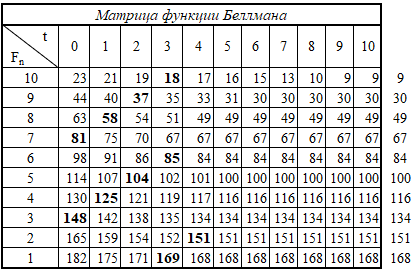
\includegraphics[scale=1]{content/images/bellman_equipment.png}
  \caption{Матрица функции Беллмана.}
  \label{fig:bellman_equipment}
\end{figure}

2 этап. Безусловная оптимизация.

В начале исследуемого десятилетнего периода возраст оборудования составляет 3 года. Находим в таблице на пересечении строки $F_1(t)$ и столбца $t=3$ значение максимальной прибыли -- $F_1(3)=169$. Найдём теперь оптимальную политику, обеспечивающую эту прибыль. Значение 169 принимает значение <<сохранения>>.  Это означает, что в начале первого года принимается решение о сохранении оборудования. К началу второго года возраст оборудования \mbox{3 + 1 = 4} года. Расположенная на пересечении строки $F_2(t)$ и столбца $t=4$ клетка принимает значения <<сохранения>>, следовательно, и второй год нужно работать на имеющемся оборудовании. К началу третьего года возраст оборудования \mbox{4 + 1 = 5} лет. Расположенная на пересечении строки $F_3(t)$ и столбца $t=5$ клетка принимает значение <<заменить>>, следовательно, в начале третьего года следует заменить оборудование. К началу четвёртого года возраст оборудования составит один год. Расположенная на пересечении строки $F_4(t)$ и столбца $t=1$ клетка принимает значение <<сохранить>>, следовательно, четвёртый год следует работать на имеющемся оборудовании. Продолжая рассуждать таким образом, последовательно, находим: $F_5(2) = 104, F_6(3) = 85, F_7(4) = 67, F_8(1) = 58, F_9(2) = 37, F_{10}(3) = 18$.

Выводы:

Итак, на оборудовании возраста 3 года следует работать 2 года, затем произвести замену оборудования, на новом оборудовании работать 3-й, 4-й, 5-й и 6-й годы, после чего произвести замену оборудования и на следующем оборудовании работать 7-й, 8-й, 9-й и 10-й годы планового периода. При этом прибыль будет максимальной и составит $F_1(3)=169$ денежных ед.



\subsection{Задача о рюкзаке}

\indent Постановка задачи: 

Дано $N$ предметов, $i$-предмет имеет массу $w_i > 0$ и стоимость $p_i > 0$. Необходимо выбрать из этих предметов такой набор, чтобы суммарная масса не превосходила заданной величины $W$ (вместимость рюкзака), а суммарная стоимость была максимальной.

Можно сформулировать данную задачу следующим образом. Пусть дано $N$ предметов, $W$ -- вместимость рюкзака, $w=(w_1,w_2, \hdots, w_N)$ -- набор положительных целых весов, $p=(p_1,p_2, \hdots, p_N)$ -- соответствующий ему набор положительных целых стоимостей. Нужно найти набор бинарных величин $B=(b_1,b_2,\hdots, b_N)$, который обеспечит максимальную стоимость рюкзака, где $b_i=1$, если предмет $i$ включён в набор, $b_i=0$, если предмет $i$ не включён.

Целевая функция задачи о рюкзаке:
\begin{equation}
    \sum_{i=1}^Nb_ip_i \longrightarrow \max
\end{equation}

Ограничения задачи о рюкзаке:
\begin{equation}
\begin{multlined}
    \sum_{i=1}^Nb_iw_i \leq W\\
    b_i \in \{0,1\} \quad \forall \; i \in \{1, \hdots, N\}
\end{multlined}
\end{equation}

Решение задачи о рюкзаке. Пусть $F(k,s)$ есть максимальная стоимость предметов, которые можно уложить в рюкзак вместимости $s$, если можно использовать только первые $k$ предметов, то есть $(n_1,n_2, \hdots, n_k)$ назовём этот набор допустимых предметов для $F(k,s)$. Исходя из этого соображения получается, что $F(k,0)=0$ и $F(0,s)=0$.

Найдём $F(k,s)$. Возможны два варианта:
\begin{enumerate}[wide]
    \item Если предмет $k$ не попал в рюкзак. Тогда $F(k,s)$ равно максимальной стоимости рюкзака с такой же вместимостью и набором допустимых предметов $(n_1,n_2, \hdots, n_{k-1})$, то есть $F(k,s)=F(k-1,s)$.
    \item Если $k$ попал в рюкзак. Тогда $F(k,s)$ равно максимальной стоимости рюкзака, где вес $s$ уменьшаем на вес $k$-ого предмета и набор допустимых предметов $(n_1,n_2, \hdots, n_{k-1})$ плюс стоимость $k$, то есть $F(k-1,s-w_k)+p_k$.
\end{enumerate}

То есть это можно представить в следующем виде:
\begin{equation}
    F(k,s) = \begin{cases}
                    F(k-1,s) & b_k=0\\
                    F(k-1,s-w_k)+p_k & b_k=1
                \end{cases}
\end{equation}


Получается, что: $F(k,s)=\max\{F(k-1, s),F(k-1,s-w_k)+p_k\}$. Стоимость искомого набора равна $F(N,W)$, так как нужно найти максимальную стоимость рюкзака, где все предметы допустимы и вместимость рюкзака $W$.

После того как мы определили максимальную стоимость рюкзака нужно восстановить предметы, которые будут входить в искомый рюкзак. Будем определять входит ли предмет $i$ в искомый набор. Начинаем с предмета $F(i,w)$, где $i=N$, $w=W$. Для этого сравниваем $F(i,w)$ со следующими значениями:
\begin{enumerate}[wide]
    \item Максимальная стоимость рюкзака с такой же вместимостью и набором допустимых предметов $(n_1, n_2, \hdots, n_{i-1})$, то есть $F(i-1,w)$.
    \item Максимальная стоимость рюкзака с вместимостью на $w_i$ меньше и набором допустимых предметов $(n_1, n_2, \hdots, n_{i-1})$ плюс стоимость $p_i$, то есть \mbox{$F(i-1,w-w_i)+p_i$}.
\end{enumerate}

Можно заметить, что при построении $F$ мы выбирали максимум их этих значений и записывали в $F(i,w)$. Тогда будем сравнивать $F(i,w)$ с $F(i-1,w)$, если равны, тогда $i$-предмет не входит в искомый набор, иначе входит.

Рассмотрим следующий пример. 

Дано $N=5$ предметов, вместимость рюкзака составляет $W=13$ и имеется следующая таблица соотношения предмета, его веса и стоимости:

\begin{table}[h]
    \centering
    \begin{tabular}{|c|c|c|}
            \hline
            Номер предмета $i$ & Вес предмета $w_i$ & Стоимость предмета $p_i$\\
            \hline
            1 & 3 & 1\\
            \hline
            2 & 4 & 6\\
            \hline
            3 & 5 & 4\\
            \hline
            4 & 8 & 7\\
            \hline
            5 & 9 & 6\\
            \hline
    \end{tabular}
    \caption{Данные для задачи о рюкзаке.}
\end{table}

Решение: 

1 этап. Условная оптимизация. 

Для начала составим матрицу функции Беллмана, она будет выглядеть следующим образом:

\begin{figure}[h]
  \centering 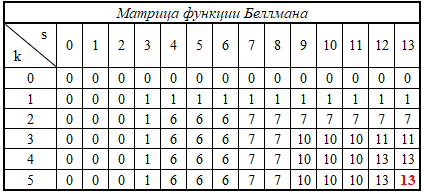
\includegraphics[scale=1]{content/images/bellman_knapsack.png}
  \caption{Матрица функции Беллмана.}
  \label{fig:bellman_knapsack}
\end{figure}

Числа от 0 до 13 в первой строчке обозначают вместимость рюкзака. Во второй строке, как только вместимость рюкзака $s\geq3$, в рюкзак добавляется 1 предмет. Далее мы просто по формуле функции Беллмана рассчитываем оставшиеся элементы и в конечном итоге получается, что стоимость рюкзака $F(5,13)=13$.

2 этап. Безусловная оптимизация.

Начинаем с клетки $F(5,13)=13$, сравниваем $F(5,13)$ и $F(4,13)$, получается $F(5,13)=F(4,13)$, следовательно переходим к клетке $F(4,13)$. Сравниваем $F(4,13)$ и $F(3,13)$, $F(4,13)>F(3,13)$, значит берём в набор 4 предмет и перемещаемся к ячейке $F(3,5)$. Продолжаем данный процесс до тех пор, пока значение функции не будет равно нулю. Пройдя данный этап, получилось, что в рюкзак пойдут 2 и 4 предметы.

\begin{figure}[h]
  \centering 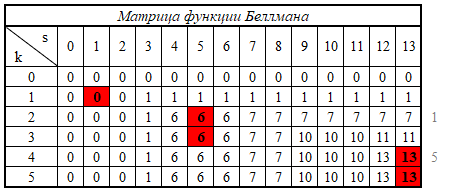
\includegraphics[scale=1]{content/images/opt_knapsack.png}
  \caption{Нахождение предметов, которые обеспечивают оптимум.}
  \label{fig:opt_knapsack}
\end{figure}

Таким образом, в набор входит 2 и 4 предмет, стоимость рюкзака составит 13, а вес рюкзака составит 12.

Так же хочется добавить, что данную задачу можно модифицировать и получить задачу о загрузке транспортного средства или задачу о целочисленном рюкзаке. Она будет формулироваться следующим образом.

Предположим, что имеется транспортное средство загружаемое $N$ различными типами предметов с весом $w_i$ и стоимостью $p_i$. Максимальная грузоподъёмность равна $W$. Определить максимальную стоимость груза, вес которого не более $W$.

Математическая постановка задачи формулируется следующим образом.

Целевая функция задачи о загрузке транспортного средства:
\begin{equation}
    \sum_{i=1}^Nx_ip_i \longrightarrow \max
\end{equation}

Ограничения задачи о загрузке транспортного средства:
\begin{equation}
\begin{multlined}
    \sum_{i=1}^Nx_iw_i \leq W\\
    x_i \in \mathbb{Z} \quad \forall \; i \in \{1, \hdots, N\}
\end{multlined}
\end{equation}



\subsection{Задача о распределении инвестиций}

\indent Постановка задачи: 

В производственное объединение входят $N$ предприятий $\textup{П}_1, \textup{П}_2, \hdots, \textup{П}_N$. Руководство объединения решило инвестировать в свои предприятия $M$ условных единиц в общей сумме. Проведённые маркетинговые исследования прогнозируют величину ожидаемой прибыли каждого из предприятий в зависимости от объёма инвестированных средств. Требуется найти такое распределение инвестиций между предприятиями, которое обеспечило бы максимум суммарной ожидаемой прибыли.

Рассмотрим следующий пример.

Инвестор выделяет средства в размере 5 условных единиц, которые должны быть распределены между тремя предприятиями. Известны значения прироста прибыли в каждом из трёх предприятий. Требуется составить план распределения инвестиций, максимизирующий общий прирост прибыли. Считается, что при нулевых инвестициях ожидается нулевая прибыль.


\begin{table}[h]
    \centering
    \begin{tabular}{|C{4cm}|C{2cm}|C{2cm}|C{2cm}|}
            \hline Инвестируемые средства (усл. ед.) & \multicolumn{3}{c|}{Прирост прибыли (усл. ед.)} \\
            \cline{2-4}
            \hline
            $x$ & $\textup{П}_1(x)$ & $\textup{П}_2(x)$ & $\textup{П}_3(x)$ \\
            \hline
            1 & 3,22 & 3,33 & 4,27 \\
            \hline
            2 & 3,57 & 4,87 & 7,64 \\
            \hline
            3 & 4 & 5,26 & 10,25 \\
            \hline
            4 & 4,12 & 7,34 & 15,93 \\
            \hline
            5 & 4,85 & 9,49 & 16,12\\
            \hline
    \end{tabular}
    \caption{Данные для задачи о распределении инвестиций.}
\end{table}

Решение: 

Число шагов в данной задаче равно 3. Пусть $S$ -- количество средств, имеющихся в наличии перед данным шагом, и характеризующих состояние системы на каждом шаге. Управление на $i$-ом шаге выберем $x$ -- количество средств, инвестируемых в $i$-ое предприятие. Выигрыш $\textup{П}_i(x_i)$ на $i$-ом шаге -- это прибыль, которую приносит $i$-ое предприятие при инвестировании в него средств $x_i$. Если через выигрыш в целом обозначить общую прибыль $W$, то он будет выглядеть следующим образом.
\begin{equation}
    W = \textup{П}_1(x_1) + \textup{П}_2(x_2) + \textup{П}_3(x_3)
\end{equation}

Если в наличии имеются средства в количестве $S$ условных единиц и в $i$-ое предприятие инвестируется $x$ условных единиц, то для дальнейшего инвестирования остаётся $(S-x)$ условных единиц. Таким образом, если на $i$-ом шаге система находилась в состоянии $S$ и выбрано управление $x$, то на $(i+1)$-шаге система будет находиться в состоянии $(S-x)$, и, следовательно, функция перехода в новое состояние имеет вид: $F_i(S-x) = S-x$.

На последнем $i$-ом шаге оптимальное управление соответствует количеству средств, имеющихся в наличии, а выигрыш равен доходу, приносимым последним предприятием.

Согласно принципу оптимальности Беллмана, управления на каждом шаге нужно выбирать так, чтобы оптимальной была сумма выигрышей на всех оставшихся до конца процесса шагах, включая выигрыш на данном шаге. Тогда функциональное уравнение Беллмана примет вид:
\begin{equation}
    W_i(S) = \max_{x \leq S}\{\textup{П}_i(x)+W_{i+1}(S-x)\}
\end{equation}

Проведём пошаговую оптимизацию, по результатам которой заполним таблицу.
\begin{figure}[h]
  \centering 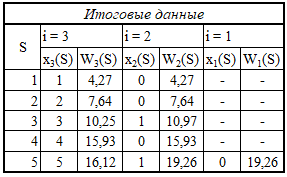
\includegraphics[scale=1]{content/images/opt_investing.png}
  \caption{Итоговые данные.}
  \label{fig:opt_investing}
\end{figure}

В первой колонке таблицы записываются возможные состояния системы, в верхней строке -- номера шагов с оптимальным управлением и выигрышем на каждом шаге, начиная с последнего. Так как для последнего шага $i=3$ функциональное уравнение Беллмана примет вид: $x_3(S)=S$, $W_3(S)=\textup{П}_3(S)$, то две колонки таблицы, соответствующие $i=3$, заполняются автоматически по таблице исходных данных.

На шаге $i=2$ основное функциональное уравнение примет вид: $W_2(S)=\max_{x \leq S} \{\textup{П}_2(x)+W_3(S-x)\}$. Поэтому для проведения оптимизации на этом шаге заполним соответствующую таблицу для различных состояний $S$ при шаге $i=2$.

\newpage

\begin{figure}[h]
  \centering 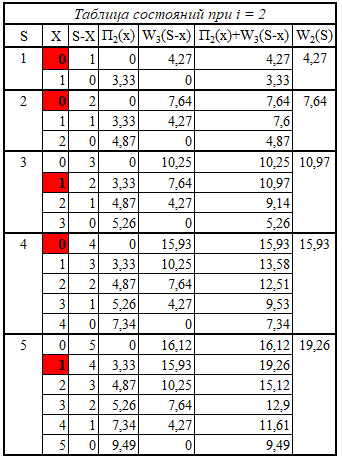
\includegraphics[scale=0.8]{content/images/opt_investing2.png}
  \caption{Таблица состояния на 2 шаге.}
  \label{fig:opt_investing2}
\end{figure}

На шаге $i=1$ основное функциональное уравнение примет вид: $W_1(S)=\max_{x \leq S}\{\textup{П}_1(x)+W_2(S−x)\}$, а состояние системы перед первым шагом $S=5$, поэтому для проведения оптимизации на этом шаге заполним соответствующую таблицу.

\begin{figure}[h]
  \centering 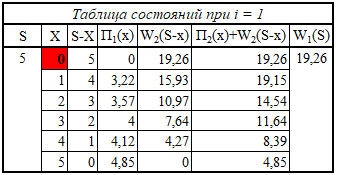
\includegraphics[scale=1]{content/images/opt_investing3.png}
  \caption{Таблица состояния на 1 шаге.}
  \label{fig:opt_investing3}
\end{figure}

Видно, что наибольшее значение выигрыша составляет 19,26. При этом оптимальное управление на первом шаге составляет $x_1(S_1)=0$ при этом $S_1=5$, на втором шаге $x_2(S_2)=1$ при этом $S_2=S_1-x_1=5$ и на третьем шаге $x_3(S_3)=4$ при этом $S_3=S_2-x_3=4$. Это означает, что  (0,1,4) -- оптимальный план распределения инвестиций между предприятиями.

Таким образом, для получения наибольшей общей прибыли в размере 19,26 условных единиц, необходимо вложить 0 условных единиц в первое предприятие, 1 условную единицу во второе предприятие и 4 условные единицы в третье предприятие.

В результате было рассмотрено три оптимизационных производственных задачи, также они были решены аналитически методом динамического программирования.
